% This is a default-selection of plugins that are used widely in this repo.

\documentclass[a4paper,10pt,fleqn]{article}
\usepackage[utf8]{inputenc}

% deutsche Trennmuster etc.
\usepackage[ngerman]{babel}
\usepackage[T1]{fontenc}

% mathematical simbols and fonts
\usepackage{mathtools} 
\usepackage{amssymb}
\usepackage{amsmath}
\usepackage{ntheorem}
\usepackage{polynom}
\usepackage{marvosym}
\usepackage{tabu}
\renewcommand*{\bmod}{\mathbin{\%}}
\everymath{\displaystyle}

\usepackage{multicol}
\usepackage{color}
\usepackage[usenames,dvipsnames]{xcolor}
\setlength{\columnsep}{1cm}
\setlength{\columnseprule}{0.25pt}
\def\columnseprulecolor{\color{gray}}
\usepackage{hyperref}

\usepackage[margin=1.5cm]{geometry}
\usepackage{graphicx}
\usepackage{pgfplots}
\pgfplotsset{compat=1.10}

%Code higlighting

\usepackage{minted}

% make lists more compact:
\newlength{\wideitemsep}
\setlength{\wideitemsep}{.5\itemsep}
\addtolength{\wideitemsep}{-5pt}
\let\olditem\item
\renewcommand{\item}{\setlength{\itemsep}{\wideitemsep}\olditem}
\renewcommand{\arraystretch}{1.25}

\title{Zusammenfassung ExEv}
\author{Fabian Hauser}
 
\begin{document}
\maketitle

\section{Einführung Experimente}

\subsection{Wissenserwerb druch Experimente nach Shewhart}
\begin{enumerate}
	\item	Hypothese formulieren
	\item	Daten im Experiment gewinnen
	\item	Hypothese Prüfen
	\item	Gegebenenfalls Modell anpassen
\end{enumerate}

\subsection{Versuchsaspekte}
\paragraph{Grössen}
\begin{itemize}
	\item	Komplexität			(Faktoren, Elemente)
	\item	Kompliziertheit		(Unbekannte oder unverstandene Zusammenhänge, oversimplification)
	\item	Rauschen, Dynamik	(keine Wiederholbarkeit, Zeitliche Variation)
\end{itemize}

\begin{description}
	\item[Validierung] \hfill \\
		Bestätigung des Modells im untersuchten Wertebereich. "Mach ich das richtige?"
	\item[Verifikation] \hfill \\
		Formaler Beweis, dass die Implementation gemäss dem Modell implementiert ist. "Mache ich es richtig?"
\end{description}

\subsection{Prozessmodell}

	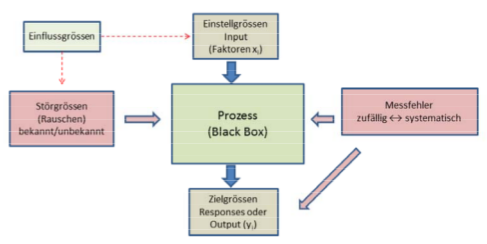
\includegraphics[scale=0.75]{img/prozessmodell.png}

\subsection{Versuchsplanung}

\begin{itemize}
	\item	Zielgrösse / Output
	\item	Einflussgrössen
	\item	Faktoren (vermutete wesentliche Einflussgrössen)
	\item	Faktorenstufen (Werte, die Faktoren in einem Experiment annehmen)
\end{itemize}

\subsection{(Mess-)Fehler}

\begin{description}
	\item[Absolute Fehler] \hfill \\
		Messfehler in einer Masseinheit
	\item[Relative Fehler] \hfill \\
		Fehler in Prozent
	\item[Zufälliger Fehler] \hfill \\
		Fehler, welcher nicht reproduzierbar auftritt
	\item[Systematische Fehler] \hfill \\
		Fehler, welcher Systematisch auftritt (z.B. falsche Lineallänge)
\end{description}

\subsubsection{Fehlerpropagation}

	Bei Multiplikation addiert sich der relative Fehler, bei Addition addiert sich der absolute Fehler.

\subsubsection{Implizite Fehlerannahme}

Bei der Impliziten Fehlerannahme geht man von $\pm$ 0.5 bis ca. 4 Einheiten der letzten angegebenen Stelle an.

Beispiel: bei $13.5 cm$ ist der Messfehler von $\pm 0.05 cm$ bis $\pm 0.4 cm$.

\section{Statistische Grundbegriffe}

\begin{description}
	\item[Mermalsträger] \hfill \\
		Der Gegenstand der statistischen Untersuchung, z.B. Utilization, Ausfallraten, Servicedauer
	\item[Grundgesamtheit] \hfill \\
		Abgrenzungsmermale, Aufteilung in Menge der Merkmalsträger, z.B. alle Messungen eines Tages, alle Maschinen einer Werkzeughalle.
	\item[Mermal] \hfill \\
		Eigenschaften eines Merkmalträgers, die bei der statistischen Untersuchung von Interesse ist.
	\item[Merkmalswert] \hfill \\
		Der Wert, welche bei Beobachtung, Befragung anfallen und statistisch ausgewertet werden.
	\item[Skala] \hfill \\
		Instrument, mit dem die Merkmalswerte bestimmt werden. Unterschieden werden: Nominalskala, Ordinalskala,  \{Intervallskala, Verhältnisskala\}(metrische Skala / Kardinalskala)
\end{description}

\subsection{Skalen}
\begin{description}
	\item[Nominalskala] \hfill \\
		Eigenschaften eines Merkmals, geordnet nach gleichen Typen. Damit lässt sich nicht gut statistisch Rechnen.
		
	\item[Ordinalskala (Rangskala)] \hfill \\
		Es wird ein Rang festgelegt für ein bestimmtes Merkmal. Dieser ist intensitätsmässig abgestuft.
		
	\item[metrische Skala] \hfill \\
		reelle Zahlen (stetig) oder ganze Zahlen (diskret) auf einer Skala angeordnet. Metrische Skalen sind immer quantitative Merkmale.
		Wird nach Intervallskala und Verhältnisskala unterschieden.
		
	\item[Intervallskala] \hfill \\
		Der Skalenwert Null ist willkürlich gewählt, kann nicht verhältnismässig ausgewertet werden.
	
	\item[Verhältnisskala] \hfill \\
		Der Skalenwret Null entspricht dem natürlichen absoluten Nullpunkt. Negative Werte sind nicht möglich, dafür kann der verhältnismässige Abstand gemessen werden.
\end{description}

\subsection{Ablauf Statistische Untersuchung}
\begin{enumerate}
	\item	Datenerhebung
		\begin{itemize}
			\item	Abgrenzung, Festlegen Untersuchungsmerkmale, Festlegung Datenumfang, erwartete Ergebnisse
			\item	Erhebungstechniken (Messungen, Zählungen, Befragungen, Beobachtungen)
			\item	Herkunft der Daten (Primärstatistik (Erhebung gezielt für Statistik), Sekundärstatistik (auf bestehender Datenbasis)
			\item Erhebungsumfang (Teil / Vollerhebung)
		\end{itemize}
	\item	Datenaufbereitung und -darstellung
		\begin{itemize}
			\item Unstrukturierte Daten aufbereiten (Strichliste, Häufigkeitstabellen, Sortierung nach Merkmalen)
		\end{itemize}
	\item	Datenanalyse
		\begin{itemize}
			\item Einfache Häufigkeitsverteilung (absolut / relativ)
			\item Komulierte Häufigkeitsverteilung, d.h. korrelieren/summieren mehrerer Häufigkeiten (dazuzählen vorangehender Häufigkeiten)
			\item Tabellarische Darstellung der Häufigkeitsbeschreibung
		\end{itemize}
	\item	Dateninterpretation
\end{enumerate}

Zu erheben sind insbesondere:
\begin{itemize}
	\item Merkmale (Faktoren)
	\item Merkmalsträgern
	\item welche Technik zur Erhebung
	\item welche Aufbereitungsverfahren
	\item welche Formen der Darstellung
	\item welche statistischen Analyseverfahren
\end{itemize}

\subsubsection{Datenerhebung}
	

\end{document}